\documentclass[12pt]{../style-files/ociamthesis}
 
\usepackage{amssymb}
\usepackage{titlesec}
\usepackage{amsmath}
\usepackage{float}
\usepackage{graphicx}
\usepackage{caption}
\usepackage{subfig}
\usepackage{xcolor}
\usepackage[section]{placeins}
\usepackage{mathrsfs}
\usepackage{bm}
\usepackage{stmaryrd}
\usepackage{siunitx}
\usepackage{rotating}
\usepackage[utf8]{inputenc}
\usepackage[round]{natbib}
\usepackage{tikz}
\usetikzlibrary{fadings}
\usetikzlibrary{snakes}

\usepackage{geometry}
 \geometry{
 a4paper,
 left=40mm,
 right=30mm,
 top=30mm,
 bottom=30mm
 }

\definecolor{theblue}{HTML}{0000CD}

% disable this package for printed version
\usepackage[colorlinks=true, linktocpage=true, allcolors=theblue]{hyperref}

\titleformat{\chapter}[display]
  {\bfseries\Large}
  {\filright\MakeUppercase{\chaptertitlename} \Large\thechapter}
  {1ex}
  {}
  [\vspace{1ex} \hrule \vspace{1pt} \hrule]

\newcommand{\adv}{    {\it Adv. Space Res.}} 
\newcommand{\annG}{   {\it Ann. Geophys.}} 
\newcommand{\aap}{    {\it Astron. Astrophys.}}
\newcommand{\aaps}{   {\it Astron. Astrophys. Suppl.}}
\newcommand{\aapr}{   {\it Astron. Astrophys. Rev.}}
\newcommand{\ag}{     {\it Ann. Geophys.}}
\newcommand{\aj}{     {\it Astron. J.}} 
\newcommand{\apj}{    {\it Astrophys. J.}}
\newcommand{\apjl}{   {\it Astrophys. J. Lett.}}
\newcommand{\apss}{   {\it Astrophys. Space Sci.}} 
\newcommand{\cjaa}{   {\it Chin. J. Astron. Astrophys.}} 
\newcommand{\gafd}{   {\it Geophys. Astrophys. Fluid Dyn.}}
\newcommand{\grl}{    {\it Geophys. Res. Lett.}}
\newcommand{\ijga}{   {\it Int. J. Geomagn. Aeron.}}
\newcommand{\jastp}{  {\it J. Atmos. Solar-Terr. Phys.}} 
\newcommand{\jgr}{    {\it J. Geophys. Res.}}
\newcommand{\mnras}{  {\it Mon. Not. Roy. Astron. Soc.}}
\newcommand{\na}{     {\it New Astronomy}}
\newcommand{\nat}{    {\it Nature}}
\newcommand{\pasp}{   {\it Pub. Astron. Soc. Pac.}}
\newcommand{\pasj}{   {\it Pub. Astron. Soc. Japan}}
\newcommand{\pre}{    {\it Phys. Rev. E}}
\newcommand{\solphys}{{\it Solar Phys.}}
\newcommand{\sovast}{ {\it Soviet  Astron.}} 
\newcommand{\ssr}{    {\it Space Sci. Rev.}}
\newcommand{\caa}{    {\it Chinese Astron. Astrohpys.}} 
\newcommand{\apjs}{   {\it Astrophys. J. Suppl.}}

\begin{document}

\baselineskip=18pt

\setcounter{secnumdepth}{3}
\setcounter{tocdepth}{3}

\setcounter{chapter}{1}


%------------------------------------------------------------------------------
\chapter{Asymmetric waveguides - eigenvalue problem}
\label{chap: EVP}
%------------------------------------------------------------------------------

%------------------------------------------------------------------------------
\section{Chapter introduction}
\label{sec: EVP intro}
%------------------------------------------------------------------------------



%------------------------------------------------------------------------------
\section{Asymmetric slab in a non-magnetic environment}
\label{sec: EVP non-mag}
%------------------------------------------------------------------------------

\subsection{Model description}
The simplest model of an asymmetric waveguide is an asymmetric magnetic slab in a non-magnetic environment\footnote{More precisely, the simplest model of an asymmetric MHD waveguide is an interface between different plasmas; the asymmetric slab is the simplest asymmetric waveguide that can oscillate in a collective body mode (see Section~\ref{sec: body}).}. Figure~\ref{fig:eq} illustrates the construction of this mathematical model, where a three-dimensional, unbounded, inviscid plasma is separated into three regions by two parallel planar interfaces at $x = \pm x_0$. The magnetic field is in the $z$-direction and has magnitude
\begin{equation}
	B(x)=
	\begin{cases}
		B_1 & \text{if } x < -x_0, \\
		B_0 & \text{if } |x|\leq{x_0}, \\
		B_2 & \text{if } x > x_0,
	\end{cases}
\end{equation}
where $B_j$, for $j = 0, 1, 2$ are constant. In the present case, we let $B_1 = B_2 = 0$ so that the plasma in the environment is non-magnetic. Within each region, denoted by subscripts 0, 1, and 2, the plasma is uniform and the equilibrium plasma pressure, density, and temperature are denoted by $p_j$, $\rho_j$, and $T_j$, respectively, for $j = 0, 1, 2$.

\begin{figure}
	\centering
	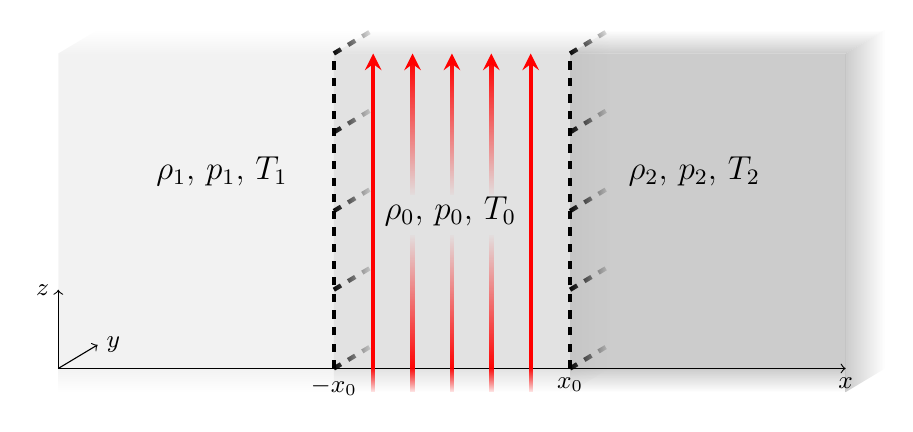
\begin{tikzpicture}
	\path [fill=lightgray, opacity=0.45] (3.5,0) -- (3.5,4) -- (6.5,4) -- (6.5,0) -- (3.5,0);
	\shade[left color=lightgray,right color=white, opacity=0.45] (6.5,0) -- (6.5,4) -- (7,4.3) -- (7,0.3) -- (6.5,0);
	\shade[top color=lightgray,bottom color=white, opacity=0.45] (3.5,0) -- (6.5,0) -- (6.5,-0.3) -- (3.5,-0.3) -- (3.5,0);
	\shade[top color=white,bottom color=lightgray, opacity=0.45] (3.5,4) -- (4,4.3) -- (7,4.3) -- (6.5,4) -- (3.5,4);
	\shade[left color=lightgray,right color=white, opacity=0.45] (6.5,0) -- (6.5,-0.3) -- (7,0) -- (7,0.3) -- (6.5,0);
	
	\path [fill=lightgray, opacity=0.8] (6.5,0) -- (6.5,4) -- (10,4) -- (10,0) -- (6.5,0);
	\shade[top color=lightgray,bottom color=white, opacity=0.8] (6.5,0) -- (10,0) -- (10,-0.3) -- (6.5,-0.3) -- (6.5,0);
	\shade[top color=white,bottom color=lightgray, opacity=0.8] (6.5,4) -- (7,4.3) -- (10.5,4.3) -- (10,4) -- (6.5,4);
	\shade[left color=lightgray,right color=white, opacity=0.8] (10,-0.3) -- (10,4) -- (10.5,4.3) -- (10.5,0) -- (10,-0.3);
	
	\path [fill=lightgray, opacity=0.2] (0,0) -- (0,4) -- (3.5,4) -- (3.5,0) -- (0,0);
	\shade[top color=lightgray,bottom color=white, opacity=0.2] (0,0) -- (3.5,0) -- (3.5,-0.3) -- (0,-0.3) -- (0,0);
	\shade[top color=white,bottom color=lightgray, opacity=0.2] (0,4) -- (0.5,4.3) -- (4,4.3) -- (3.5,4) -- (0,4);
	
	\draw [<->] (0,1) -- (0,0) -- (10,0);
	\draw [->] (0,0) -- (0.5,0.3);
	
	\draw [ultra thick, dashed] (3.5,0) -- (3.5,4);
	\draw [ultra thick, dashed, path fading=east] (3.5,0) -- (4,0.3);
	\draw [ultra thick, dashed, path fading=east] (3.5,4) -- (4,4.3);
	\draw [ultra thick, dashed, path fading=east] (3.5,2) -- (4,2.3);
	\draw [ultra thick, dashed, path fading=east] (3.5,1) -- (4,1.3);
	\draw [ultra thick, dashed, path fading=east] (3.5,3) -- (4,3.3);
	\draw [ultra thick, red, -stealth] (4,0) -- (4,4);
	\draw [ultra thick, red, path fading=south] (4,-0.3) -- (4,0);
	\draw [ultra thick, red, path fading=north] (4.5,0) -- (4.5, 1.7);
	\draw [ultra thick, red, path fading=south] (4.5,-0.3) -- (4.5,0);
	\draw [ultra thick, red, path fading=south] (4.5,2.2) -- (4.5,3.9);
	\draw [ultra thick, red, -stealth] (4.5,3.9) -- (4.5,4);
	\draw [ultra thick, red, path fading=north] (5,0) -- (5, 1.7);
	\draw [ultra thick, red, path fading=south] (5,-0.3) -- (5, 0);
	\draw [ultra thick, red, path fading=south] (5,2.2) -- (5,3.9);
	\draw [ultra thick, red, -stealth] (5,3.9) -- (5,4);
	\draw [ultra thick, red, path fading=north] (5.5,0) -- (5.5, 1.7);
	\draw [ultra thick, red, path fading=south] (5.5,-0.3) -- (5.5, 0);
	\draw [ultra thick, red, path fading=south] (5.5,2.2) -- (5.5,3.9);
	\draw [ultra thick, red, -stealth] (5.5,3.9) -- (5.5,4);
	\draw [ultra thick, red, -stealth] (6,0) -- (6,4);
	\draw [ultra thick, red, path fading=south] (6,-0.3) -- (6,0);
	\draw [ultra thick, dashed] (6.5,0) --(6.5,4);
	\draw [ultra thick, dashed, path fading=east] (6.5,0) -- (7,0.3);
	\draw [ultra thick, dashed, path fading=east] (6.5,4) -- (7,4.3);
	\draw [ultra thick, dashed, path fading=east] (6.5,2) -- (7,2.3);
	\draw [ultra thick, dashed, path fading=east] (6.5,1) -- (7,1.3);
	\draw [ultra thick, dashed, path fading=east] (6.5,3) -- (7,3.3);
	
	\small
	\node [below] at (3.5,0) {$-x_0$};
	\node [below] at (6.5,0) {$x_0$};
	\node [below] at (10,0) {$x$};
	\node [left] at (0,1) {$z$};
	\node [right] at (0.5,0.3) {$y$};
	
	\large
	\node [right] at (1.1,2.5) {$\rho_1$, $p_1$, $T_1$};
	\node [right] at (4,2) {$\rho_0$, $p_0$, $T_0$};
	\node [right] at (7.1,2.5) {$\rho_2$, $p_2$, $T_2$};
	\end{tikzpicture}
	\caption{The equilibrium state inside the slab, ($|x| \leq x_0$) and outside the slab, ($x < -x_0$ and $x > x_0$). The red arrows illustrate magnetic field lines, $B(x)\mathbf{\widehat{z}}$, and the dashed black lines indicate the boundaries of the slab.}
	\label{fig:eq}
\end{figure}

To ensure that the model is in equilibrium, the total pressure in each external region must balance the total pressure in the internal region, namely
\begin{equation}
	p_1 = p_0 + \frac{B_0^2}{2\mu_0} = p_2, \label{pressure balance}
\end{equation}
where $\mu_0$ is the permeability of free space. Defining the sound speed in each region by $c_j=\sqrt{\gamma p_j/\rho_j}$ for $j = 0, 1, 2$, where $\gamma$ is the adiabatic index\footnote{The adiabatic index is assumed uniform across the whole domain under the single-fluid approximation.}, we can rewrite Equation~\eqref{pressure balance} as
\begin{equation}
\frac{c_1^2}{c_2^2}=\frac{\rho_2}{\rho_1}. \label{sound speeds}
\end{equation}







The effects of gravity are ignored throughout; it is important to note, however, that equilibrium density stratification itself in the solar atmosphere can be a consequence of gravity, but gravity can be ignored if the gravity scale height is large compared to the wavelength and the thickness of the magnetic slab, which is safe to assume for many small-scale solar atmospheric structures.





\subsection{The dispersion relation}

\subsubsection{Derivation}

\subsubsection{First-order symmetric slab}

\subsection{Analytical solutions}

\subsubsection{Spurious solutions}

\subsubsection{Limiting case - incompressible plasma}

\subsubsection{Limiting case - zero-beta}

\subsubsection{Limiting case - thin slab}

\subsubsection{Limiting case - wide slab}

\subsection{Numerical solutions}

\subsubsection{Varying the degree of asymmetry}

\subsection{Eigenfunctions}

\subsubsection{Analogy to coupled spring and mass oscillator}
Actually do the maths for this.


%------------------------------------------------------------------------------
\section{Asymmetric slab in a magnetic environment}
\label{sec: EVP mag}
%------------------------------------------------------------------------------

\subsection{Model description}

\subsection{The dispersion relation}

\subsection{Implications for observations}

\subsubsection{Quasi-symmetric modes}

\subsubsection{Asymmetric mode or superposition of symmetric modes?}
Table of observable indicators of each case.

\subsubsection{Possible alternative causes of observed asymmetry}
Possibilities: 
\begin{itemize}
	\item Asymmetric ICs
	\item Non-collective oscillations
	\item Observational artefact
\end{itemize}
Include discussion about how to differentiate between these.



\bibliographystyle{plainnat}
\bibliography{../main/references}  

\end{document}
